\documentclass[11pt]{article}
\usepackage[margin=1in]{geometry}
\usepackage{volfit_preamble}
\graphicspath{{figures/}}

\title{\textbf{Calendar-Arbitrage Prevention}\\[2pt]
\large Convex order, integrated quantiles, and a model-agnostic soft hinge\\[2pt]
\normalsize Vol-Fitter Technical Notes, No.~10}
\author{Vol-Fitter}
\date{\today}

\begin{document}
\maketitle
% Auto-generated by gen_calendar.py — do not edit.
\newcommand{\calviolfree}{0.0059}
\newcommand{\calviolcured}{4.58e-07}
\newcommand{\calstride}{25}


\begin{abstract}
Butterfly-freedom keeps a single smile a valid density; calendar-freedom keeps a
\emph{surface} consistent across maturities. This note documents how the
Vol-Fitter enforces it. With every expiry normalized by its forward, absence of
calendar arbitrage is the statement that the terminal laws are increasing in
convex order --- equivalently, that normalized call prices, and hence total
implied variance at each fixed log-moneyness, are non-decreasing in maturity. We
give two enforcements. For LQD the convex order is exactly an ordering of the
\emph{integrated upper-quantile} curves, which each built slice already carries as
its asset-share integral, so the constraint is an elementwise array comparison
with no quantile inversion; expiries are fitted nearest-to-farthest under a soft
slack. For the SVI and Multi-Core SIV overlays, which carry no quantile curve, a
\emph{model-agnostic} hinge enforces $w_{\text{far}}(k)\ge w_{\text{near}}(k)$
directly on total variance. We then explain the subtle but important
\emph{confinement} fix --- the floor must be sampled only on the traded strike
range, or a steep short-dated slice's linear-wing extrapolation manufactures a
phantom violation that flattens the in-data fit. A worked example takes an
inverted-wing pair from a calendar violation of \calviolfree\ to \calviolcured.
\end{abstract}

\tableofcontents
\newpage

%======================================================================
\section{What calendar-freedom means}
\label{sec:meaning}

Fix log-moneyness $k$ and let $C_{T}(k)$ be the forward-normalized call at expiry
$T$. With all expiries normalized to unit forward, the absence of a calendar
spread arbitrage is
\begin{equation}
C_{T_i}(k)\le C_{T_j}(k)\quad\text{for }T_i<T_j,\ \forall k,
\label{eq:calmono}
\end{equation}
i.e.\ a longer-dated call is never cheaper than a shorter-dated one at the same
moneyness. Because the Black price is increasing in total variance, under
deterministic proportional carry \eqref{eq:calmono} is equivalent to total
variance being non-decreasing in maturity, $w_{T_i}(k)\le w_{T_j}(k)$. The
sharper, model-independent statement is in terms of the terminal laws: writing
$Y_T=S_T/F_T$ (mean one), \eqref{eq:calmono} holds iff
\begin{equation}
Y_{T_i}\le_{cx}Y_{T_j},
\label{eq:convex}
\end{equation}
the $Y$'s are increasing in \emph{convex order}. This is the object the LQD
enforcement uses directly.

\begin{heuristic}
Convex order with equal means says the longer-maturity law is a ``mean-preserving
spread'' of the shorter one: same forward, more dispersion. That is exactly what a
diffusion does --- variance accumulates with time --- so calendar-freedom is the
statement that the surface is consistent with \emph{some} martingale, even if the
fitter never names one. Enforcing it on the fitted slices is what stops two
independently-fitted expiries from implying a negative forward variance between
them.
\end{heuristic}

%======================================================================
\section{The LQD-exact enforcement}
\label{sec:lqd}

\subsection{Convex order as integrated quantiles}

For equal-mean laws, $Y_{T_i}\le_{cx}Y_{T_j}$ holds iff the \emph{integrated
upper-quantile} curves are ordered:
\begin{equation}
G_i(\alpha):=\int_\alpha^1 Q_{Y,T_i}(u)\,\dd u\ \le\ G_j(\alpha)\quad\forall\alpha\in[0,1],
\label{eq:Gorder}
\end{equation}
with equality at $\alpha=0$ (equal means). Now recall (Note~01) that for an LQD
slice $Q_Y(u)=e^{Q(u)}$ and, in the logit coordinate, $\dd u=u(1-u)\,\dd z$, so
\begin{equation}
G(\alpha)=\int_{\alpha}^1 e^{Q(u)}\,\dd u=\int_{z_\alpha}^{\infty}e^{Q(z)}\Lambda(z)(1-\Lambda(z))\,\dd z=A(z_\alpha),
\end{equation}
which is \emph{exactly} the asset-share integral $A(z)$ every built slice already
carries on the shared quadrature grid. The calendar constraint is therefore an
elementwise comparison of two \texttt{a\_z} arrays --- no quantile inversion, no
per-strike call comparison --- and, because the grid is uniform in $z$, it places
constraint points densely in the wings exactly where they matter.

\subsection{Sequential fitting with slack}

The surface is built nearest-to-farthest. The constraint subgrid takes every
\calstride th node ($\sim320$ points on the $8001$-node grid). Each new slice is
fitted subject to the soft floor
\begin{equation}
A_j(z_m)\ \ge\ A_i(z_m)-\tau_m,
\label{eq:slack}
\end{equation}
implemented as the squared-hinge slack $\sqrt{W_{\text{cal}}}\,\max(A_i(z_m)-A_j(z_m),0)$
in the LQD objective (weight \texttt{calendarWeight}, default $10^6$). The floor is
keyed on the constraint $z$-\emph{coordinates}, so the next slice can enforce it by
Hermite-evaluating its own curve there even when it is calibrated on a coarser
optimization grid --- bit-for-bit equivalent to the node-indexed form on the native
grid.

%======================================================================
\section{The model-agnostic enforcement}
\label{sec:agnostic}

The SVI and Multi-Core SIV overlays carry no integrated-quantile curve, so they use
Gatheral's equivalent \emph{surface} condition directly: total implied variance
non-decreasing in maturity,
\begin{equation}
w_{\text{far}}(k)\ \ge\ w_{\text{near}}(k)\quad\forall k,
\label{eq:wfloor}
\end{equation}
enforced as a soft hinge $\sqrt{W_{\text{cal}}}\,\max(w_{\text{near}}(k)-w_{\text{far}}(k),0)$
on a log-moneyness grid. This reads only the previous slice's $\text{implied\_w}(k)$,
so it applies to \emph{any} model --- raw SVI, Multi-Core SIV, or the local-vol
overlay --- and gives the whole surface a uniform calendar treatment regardless of
which model draws each slice. As residual rows it is one line, the same squared-hinge
shape as the band objective (Note~07):

\begin{lstlisting}[caption={The model-agnostic calendar hinge \eqref{eq:wfloor}
(distilled from \texttt{calib/calendar.py}).},label={lst:cal}]
def calendar_residual(w_far, w_near, weight):    # w_* = implied_w(k) on the SAME grid
    return np.sqrt(weight) * np.maximum(w_near - w_far, 0.0)   # 0 unless the later dips below
\end{lstlisting}

\subsection{The confinement fix}
\label{sec:confine}

Where the floor \eqref{eq:wfloor} is \emph{sampled} turns out to be critical.

\begin{caution}
If the floor grid is fixed and wide (say $k\in[-1,1]$, far beyond the traded
strikes), then for a family with \emph{linear wings} (SVI) a steep short-dated
slice extrapolates to far higher wing variance than a flatter long-dated one, so
$w_{\text{near}}>w_{\text{far}}$ out in the untraded wing --- a \emph{phantom}
violation created purely by extrapolation. The optimizer then flattens the
long-dated wing to ``cure'' a problem the data never posed. This was observed live
on NVDA and SPY overlays.
\end{caution}

The fix is \emph{confinement}: \texttt{variance\_floor\_grid\_from} builds the
floor grid on the \emph{observed} quote range $[\min k,\max k]$ only (empty quotes
fall back to the wide grid) --- a two-line change that is the whole cure:

\begin{lstlisting}[caption={The confinement fix: sample the floor only on the traded
range (distilled from \texttt{calib/calendar.py}).},label={lst:confine}]
def floor_grid(k_quotes, n=41):          # the grid the calendar hinge is sampled on
    return np.linspace(k_quotes.min(), k_quotes.max(), n)   # traded span, NOT a fixed wide grid
\end{lstlisting}

Calendar arbitrage is only meaningful where prices are
observable; confining the floor keeps the constraint where the fit and the data
both live, and leaves each model's wings to its own Lee-admissible extrapolation
(Note~09). This is the same lesson as the local-vol convex-wing regression of
Note~04: \emph{a no-arbitrage constraint must not be sampled where only
extrapolation lives.}

%======================================================================
\section{Worked example}
\label{sec:example}

\Cref{fig:cross} fits an \emph{inverted-wing} pair: a high-vol short expiry
($T=0.25$) over a calmer long expiry ($T=0.5$), the kind of term structure an
imminent event produces. Fitted independently, the long slice's total variance
dips \emph{below} the short one's in the wings (the shaded region) --- a calendar
violation of $\calviolfree$. Refitting the long slice under the calendar floor from
the short one lifts it to dominate everywhere, driving the violation to
$\calviolcured$ (numerically zero). \Cref{fig:G} shows the cured pair's integrated
upper-quantile curves correctly ordered, $G_{\text{far}}\ge G_{\text{near}}$ ---
the convex order \eqref{eq:convex} made manifest.

\begin{figure}[H]
\centering
\begin{minipage}{0.55\textwidth}\centering
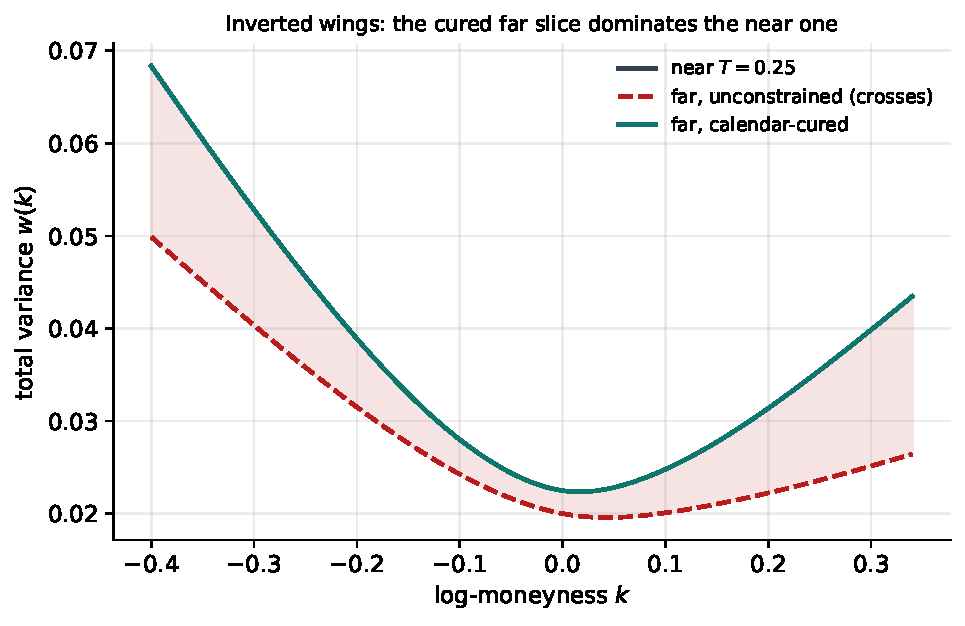
\includegraphics[width=\textwidth]{fig_cal_cross.pdf}\\[1pt]
{\footnotesize (a) total variance: crossing, then cured}
\end{minipage}\hfill
\begin{minipage}{0.42\textwidth}\centering
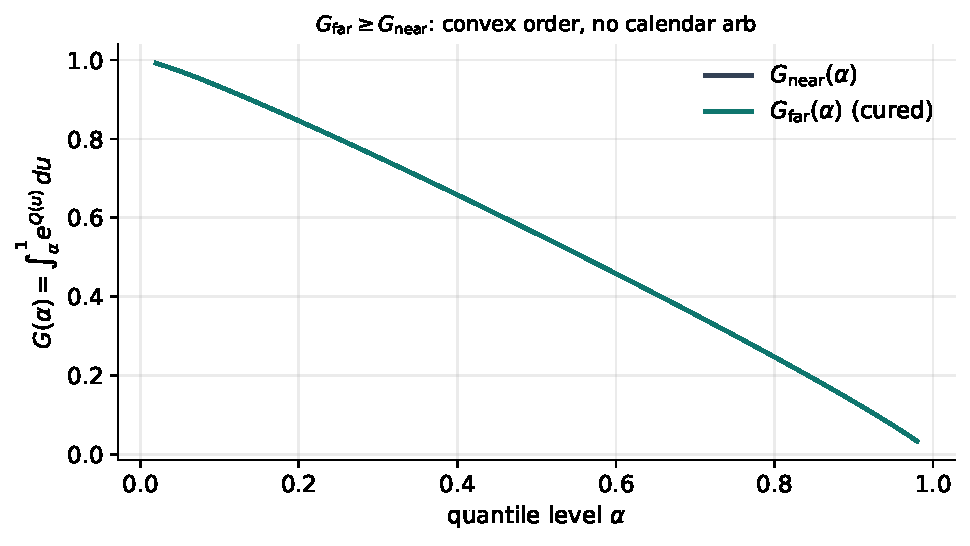
\includegraphics[width=\textwidth]{fig_cal_G.pdf}\\[1pt]
{\footnotesize (b) integrated quantiles, ordered}
\end{minipage}
\caption{An inverted-wing pair: the unconstrained long slice crosses the short one
(violation $\calviolfree$); the calendar floor cures it (violation $\calviolcured$).}
\label{fig:cross}
\end{figure}
\begin{figure}[H]\centering\phantomsection\label{fig:G}\end{figure}

%======================================================================
\section{What is original here}
\label{sec:original}

The convex-order characterization is classical (Strassen, Carr--Madan); the
contributions are implementation. Recognizing that the LQD asset-share integral
$A(z)$ \emph{is} the integrated upper-quantile curve $G(\alpha)$ makes the calendar
constraint a free elementwise comparison rather than a dense grid of inverted
call inequalities. Extending the same no-arbitrage to the SVI/SIV/LV overlays
through the model-agnostic total-variance floor \eqref{eq:wfloor} gives the whole
surface one calendar treatment. And the \emph{confinement} fix \eqref{sec:confine}
--- sampling the floor only where data lives --- is a genuinely non-obvious lesson
that the same wide-grid mistake recurs in two places (here and the local-vol
convex wing) and is cured the same way.

\appendix
%======================================================================
\section{Hyperparameter atlas}
\label{app:atlas}

\begin{longtable}{p{0.26\textwidth}p{0.14\textwidth}p{0.52\textwidth}}
\caption{Calendar-arbitrage hyperparameters.}\label{tab:atlas}\\
\toprule Knob & Default & Role\\ \midrule
\endfirsthead \toprule Knob & Default & Role\\ \midrule \endhead
\multicolumn{3}{l}{\emph{Surfaced}}\\ \midrule
\texttt{enforceCalendar} & on & Master toggle for calendar coupling.\\
\texttt{calendarWeight} $W_{\text{cal}}$ & $10^{6}$ & Soft-constraint penalty strength.\\
\midrule
\multicolumn{3}{l}{\emph{Hidden}}\\ \midrule
\texttt{CAL\_STRIDE} & $\calstride$ & LQD constraint subgrid stride ($\sim320$ points).\\
\texttt{VAR\_FLOOR\_KMIN/KMAX} & $[-1,1]$ & Fallback wide floor grid (empty quotes only).\\
\texttt{VAR\_FLOOR\_N} & $161$ & Wide floor grid resolution.\\
\texttt{VAR\_FLOOR\_N\_DATA} & $41$ & Confined floor grid resolution.\\
floor grid & traded range & \texttt{variance\_floor\_grid\_from}: confined to $[\min k,\max k]$.\\
\bottomrule
\end{longtable}

\noindent\textbf{Performance.} The LQD constraint is an array slice and subtraction
on the already-built asset share --- effectively free; its Jacobian rows are
$-\partial A/\partial\theta$ on the active constraints, supplied by the analytic
Jacobian (Note~01). The model-agnostic floor is $\sim40$ arithmetic evaluations of
the previous slice's $w(k)$. Confinement \emph{reduces} work by not over-sampling
the extrapolation region.

\begin{thebibliography}{9}
\bibitem{Strassen1965} V.~Strassen. The existence of probability measures with
given marginals. \emph{Ann.\ Math.\ Statist.}, 36(2):423--439, 1965.
\bibitem{CarrMadan2005} P.~Carr and D.~Madan. A note on sufficient conditions for
no arbitrage. \emph{Finance Research Letters}, 2(3):125--130, 2005.
\bibitem{GatheralJacquier2014} J.~Gatheral and A.~Jacquier. Arbitrage-free SVI
volatility surfaces. \emph{Quantitative Finance}, 14(1):59--71, 2014.
\end{thebibliography}

\end{document}
